% Copyright (c) 2024 Ludovic Lars
% This work is licensed under the CC BY-NC-SA 4.0 International License

\chapter{Le changement de la monnaie}
\label{ch:changement}

Une monnaie est un accord concernant un moyen mutuellement acceptable dans le commerce. Cet accord peut porter sur des propriétés physiques, auquel cas le support monétaire est une marchandise, ou des propriétés numériques, auquel cas le support monétaire est un protocole informatique. Bitcoin appartient à cette seconde catégorie.

Par sa nature ouverte et libre, le code informatique de Bitcoin peut être copié, modifié et réutilisé à volonté. Par conséquent, le protocole (et la monnaie qu'il définit) peut lui aussi être changé, grâce à l'application d'un code différent sur le réseau. Bitcoin n'est ainsi pas un système figé qui serait géré par une autorité centrale, mais une structure ouverte qui connaît une évolution organique au cours du temps.

\section*{Le protocole}
\addcontentsline{toc}{section}{Le protocole}

% Nature protocolaire de Bitcoin
Bitcoin est par essence un protocole de communication informatique, c'est-à-dire un ensemble de règles permettant à différentes parties d'un réseau d'échanger des informations. Ce protocole permet aux nœuds du réseau pair à pair de s'échanger des transactions et des blocs et de se mettre d'accord sur le registre de propriété considéré comme correct. Le résultat est un système monétaire.

% Autres protocoles liés à Internet
Bitcoin se rapproche, de façon plus ou moins manifeste de protocoles existants. C'est par exemple le cas d'autres protocoles construits sur Internet, comme HTTP (\eng{HyperText Transfer Protocol}) qui est utilisé pour l'affichage des pages web, SMTP (\emph{Simple Mail Transfer Protocol}) qui est utilisé pour le courrier électronique, ou encore BitTorrent, qui permet le partage de fichiers de pair à pair. C'est également le cas des protocoles qui soutiennent Internet, appelés protocoles de la suite TCP/IP en référence aux deux premiers qui la composent~: IP (\eng{Internet Protocol}) qui assure la communication au niveau de la couche réseau, et TCP (\eng{Transmission Control Protocol}) qui assure la transmission au niveau de la couche transport, en surcouche de la couche réseau.

% Langages de programmation et langues
Plus éloigné de Bitcoin, on peut citer la catégorie des langages de programmation. Ces langages permettent d'écrire du code (texte spécifique encodé en UTF-8), qui est transformé en fichier exécutable par un compilateur (par exemple dans le cas du C, du C++ ou du Java) ou qui est directement exécuté par un interpréteur (comme c'est le cas pour Python ou Javascript). Dans le même ordre d'idées, les langues humaines comme le français ou l'anglais sont aussi des protocoles de communication, dont les règles sont moins formelles et moins bien définies, mais qui permettent aux hommes d'échanger des informations.

% Monnaies
Enfin, les monnaies peuvent être vues comme des sortes de protocole, en constituant des moyens communs de communiquer de la valeur et de formaliser l'échange économique. La monnaie se définit en particulier par le support accepté dans le commerce~: pour une marchandise comme l'or ou l'argent, ce support est un élément chimique~; pour la monnaie fiat, il s'agit d'un certificat émis par une autorité.

% Bitcoin : deux sous-protocoles
Dans le cas de Bitcoin, le protocole est formé de l'ensemble des règles qui permettent au réseau de communiquer et de se coordonner. Ce protocole se divise en deux parties distinctes~: le protocole de transmission, constitué des règles de réseau, et le protocole régissant le contenu transmis, constitué des règles de consensus.

% Règles de réseau
Les règles de réseau sont les règles qui permettent aux nœuds d'entrer en communication sur Internet. Ces règles concernent le protocole de transport sous-jacent (TCP, Tor, UDP pour FIBRE), le port réseau (8333 pour le réseau principal BTC), la procédure de découverte de pairs, la syntaxe des messages de transmission de données\pagenote{«~la syntaxe des messages de transmission de données~»~: Bitcoin Wiki, \eng{Protocol documentation: Common structures}~: \url{https://en.bitcoin.it/wiki/Protocol_documentation\#Common\_structures}.},~etc. Elles peuvent différer selon les nœuds sans briser formellement le consensus~: il suffit qu'un nœud acceptant les deux ensembles de règles fasse la liaison. De même, les nœuds sont libres de restreindre (temporairement ou définitivement) leur connexion avec un autre nœud, notamment dans le but d'éviter le spam.

% Règles de consensus
Les règles de consensus sont les règles de construction et d'organisation des blocs et des transactions. Elles régissent la validité du registre sur lequel les membres du réseau arrivent à un accord, d'où leur nom. Ces règles sont critiques~: un nœud qui transmettrait une transaction ou un bloc invalide aux autres nœuds verrait sa transaction ou son bloc être rejeté par le reste du réseau.

% Exemples
Les règles de consensus sont nombreuses. Certaines d'entre elles sont largement connues et explicites. En voici quelques-unes ici~:

\begin{itemize}
\item[$\bullet$] Le montant en entrée d'une transaction doit être supérieur (ou égal) au montant en sortie, la différence représentant les frais collectés par le mineur~;
\item[$\bullet$] Chaque entrée doit contenir un script de déverrouillage (contenant la ou les signatures) qui correspond au script de verrouillage (l'adresse d'envoi) de la sortie dépensée~;
\item[$\bullet$] Une sortie transactionnelle ne peut être dépensée qu'une seule fois, en raison de l'interdiction de double dépense~;
\item[$\bullet$] Chaque bloc doit comporter une preuve de travail, produite par hachages répétés de l'entête par la fonction SHA-256, de degré supérieur à la difficulté du réseau~;
\item[$\bullet$] La subvention dans chaque bloc doit être inférieure à une limite, qui est divisée par deux tous les 210~000 blocs (4 ans environ)~;
\item[$\bullet$] La difficulté du minage est ajustée tous les 2016 blocs (2 semaines environ), de sorte à garantir un temps moyen de 10 minutes entre chaque bloc~;
\item[$\bullet$] Le poids des blocs est limité à 4 millions d'unités de poids (telles que définies par SegWit), ce qui restreint la capacité transactionnelle du système.
\end{itemize}

Les règles de consensus sont trop nombreuses pour être toutes explicitées. Quand elles ne le sont pas, ces règles sont implicitement définies dans l'implémentation logicielle de référence, qui est Bitcoin Core dans le cas de BTC.

\section*{Les implémentations logicielles}
\addcontentsline{toc}{section}{Les implémentations logicielles}

% --- Les implémentations logicielles ---

% Implémentations complètes et partielles
Les implémentations logicielles sont les programmes informatiques qui mettent en œuvre le protocole. Dans le cas des implémentations de nœud complet, la totalité des règles de consensus sont appliquées. Les implémentations peuvent également être partielles, auquel cas elles ne mettent pas en œuvre l'intégralité des règles de consensus~: c'est par exemple le cas des portefeuilles légers, qui procèdent à une vérification simplifiée de leurs transactions.

% Implémentations dans BTC
Dans BTC, il existe plusieurs implémentations, dont Bitcoin Core, Libbitcoin, btcd et Bitcoin Knots. La plus connue est Bitcoin Core, qui est à la fois l'implémentation historique créée par Satoshi Nakamoto («~\eng{Satoshi client}~») et reprise par Gavin Andresen en 2010, l'implémentation principale utilisée par plus de 99~\% des nœuds en novembre 2023\pagenote{«~l'implémentation principale utilisée par plus de 99~\% des nœuds en novembre 2023~»~: \url{https://coin.dance/nodes}.}, et l'implémentation de référence, qui définit les règles de consensus implicites.

% Implémentations dans BCH et ETH
D'autres protocoles possèdent des implémentations différentes. Bitcoin Cash présente une multiplicité d'implémentations dont les deux principales sont Bitcoin Cash Node (l'implémentation de référence issue de Bitcoin ABC, elle-même issue de Bitcoin Core) et Bitcoin Unlimited. Ethereum repose également sur une diversité d'implémentations\pagenote{«~une diversité d'implémentations~»~: \url{https://clientdiversity.org/\#distribution}.}, qui gèrent la transmission et la vérification des transactions (Geth, Nethermind, etc.) ou celles des blocs (Prysm, Lighthouse, etc.)

% Logiciel libre
Une implémentation est en règle générale un logiciel libre, c'est-à-dire un logiciel dont le code est publié en accès libre sous une licence permettant l'utilisation, la modification et la reproduction. Cette caractéristique, technique et juridique, est \emph{essentielle} à Bitcoin, car elle permet non seulement de vérifier le fonctionnement du logiciel\sendnote{«~Le code source ouvert signifie que n'importe qui peut examiner le code de manière indépendante. S'il s'agissait d'une source fermée, personne ne pourrait vérifier la sécurité. Je pense qu'il est essentiel pour un programme de cette nature d'avoir un code source ouvert.~» -- Satoshi Nakamoto, \eng{Re: Questions about Bitcoin}, \wtime{10/12/2009 20:49:02 UTC}~: \url{https://bitcointalk.org/index.php?topic=13.msg46\#msg46}.}, mais aussi de reprendre la main sur le code dans le cas où les développeurs iraient dans une direction non désirée. % "Being open source means anyone can independently review the code.  If it was closed source, nobody could verify the security.  I think it's essential for a program of this nature to be open source."

% Fork
L'action de copier et de modifier un logiciel est appelé un \eng{fork} ou embranchement. Il s'agit de créer un nouveau logiciel à partir du code source d'un logiciel existant, dont l'existence découle d'une vision différente du développement de ce logiciel. Les distributions Linux sont ainsi formées de distributions antérieures\pagenote{«~Les distributions Linux sont ainsi formées de distributions antérieures~»~: Andreas Lundqvist, Donjan Rodic, Mohammed A. Mustafa, Muhammad Herdiansyah, Fabio Loli, \eng{Linux Distribution Timeline}, 27 février 2021~: \url{https://commons.wikimedia.org/wiki/File:Linux_Distribution_Timeline_27_02_21.svg}.}. On peut aussi citer OpenOffice.org qui a donné LibreOffice et Apache OpenOffice.

% Historique de Bitcoin Core
Bitcoin Core descend directement de la première implémentation codée par Satoshi Nakamoto et partagée publiquement par ce dernier le 8 janvier 2009. Initialement appelé simplement «~Bitcoin~», le logiciel a été renommé en bitcoind~/~Bitcoin-Qt en 2011\pagenote{«~le logiciel a été renommé en bitcoind~/~Bitcoin-Qt en 2011~»~: Gavin Andresen, \eng{Bitcoin-Qt/bitcoind version 0.5.0}, \wtime{21/11/2011 17:17:04 UTC}~: \url{https://bitcointalk.org/index.php?topic=52480.msg626275\#msg626275}.}, puis en Bitcoin Core le 19 mars 2014\pagenote{«~en Bitcoin Core le 19 mars 2014~»~: Bitcoin Core, \eng{Bitcoin Core version 0.9.0 released}, 19 mars 2014~: \url{https://bitcoin.org/en/release/v0.9.0\#rebranding-to-bitcoin-core}.}.

% Code source
Bitcoin Core est un logiciel codé en C++. Initialement hébergé sur SourceForge, le code est aujourd'hui présent sur GitHub\sendnote{\eng{Bitcoin Core integration/staging tree}~: \url{https://github.com/bitcoin/bitcoin}.}. Il est publié sous licence libre MIT, de sorte que quiconque peut le copier et le modifier à sa guise. En particulier, la licence MIT est permissive~: elle n'empêche pas la réutilisation du code comme partie ou comme base d'un logiciel soumis à une licence privative. Cette licence a été choisie par Satoshi, au détriment de la licence GPL, en raison de sa compatibilité avec les autres licences\sendnote{Satoshi Nakamoto, \eng{Re: Switch to GPL}, \wtime{12/09/2010 19:24:53 UTC}~: \url{https://bitcointalk.org/index.php?topic=989.msg12494\#msg12494}.}.

% Développement de Bitcoin Core
Le développement de Bitcoin Core se fait de manière ouverte et méritocratique. Le dépôt GitHub est ouvert à tous et n'importe qui peut contribuer au maintien et à l'amélioration du logiciel en faisant une demande de modification du code (\eng{pull request}). Les contributeurs fréquents sont appelés des «~\eng{core developers}~». Pour faciliter le développement, les contributeurs communiquent par différents moyens, mais les deux principaux sont le canal IRC bitcoin-core-dev où ont lieu la plupart des discussions et la liste de diffusion bitcoin-dev\pagenote{«~la liste de diffusion bitcoin-dev~»~: The bitcoin-dev Archives~: \url{https://lists.linuxfoundation.org/pipermail/bitcoin-dev/}.}.

% Hiérarchie
Toutefois, Bitcoin Core dispose d'une certaine hiérarchie. Le dépôt est en effet géré par des mainteneurs qui sont responsables de fusionner les demandes de modification créées par les contributeurs. L'inclusion dans le code dépend ainsi de différents critères évalués par ces mainteneurs, comme l'utilité démontrable du changement, le format correct suivant les lignes directrices du projet, la revue par les pairs ou la réputation du contributeur\sendnote{«~Les mainteneurs prendront en considération un correctif s'il est en accord avec les principes généraux du projet~; s'il répond aux normes minimales d'inclusion~; et jugeront du consensus général des contributeurs.~» -- \eng{Contributing to Bitcoin Core}, 26 mai 2023~: \url{https://github.com/bitcoin/bitcoin/blob/25.x/CONTRIBUTING.md}.}. % Maintainers will take into consideration if a patch is in line with the general principles of the project; meets the minimum standards for inclusion; and will judge the general consensus of contributors.

% Mainteneur principal
La charge du logiciel était initialement allouée à un mainteneur principal, qui avait pour rôle de nommer les mainteneurs normaux, de décider du cycle de sortie du logiciel, de fusionner l'ensemble des modifications et de modérer les débats. Cette mission était assurée au début par Satoshi Nakamoto qui s'occupait d'intégrer les contributions sur le dépôt SourceForge. Puis, le 23 février 2011, Satoshi a transmis la responsabilité à Gavin Andresen, avant de disparaître définitivement. Gavin s'est ensuite chargé du projet pendant plus de trois ans avant de laisser sa place à Wladimir J. van der Laan le 7 avril 2014. Enfin, le 7 février 2023, ce dernier a démissionné après neuf ans de service. La fonction de mainteneur principal a alors été supprimée et remplacée par la responsabilité collective des mainteneurs\sendnote{Wladimir J. van der Laan, \eng{The widening gyre}, 21 janvier 2021, archive~: \url{https://web.archive.org/web/20210121201607/https://laanwj.github.io/2021/01/21/decentralize.html}~; Wladimir J. van der Laan, \eng{Remove laanwj from trusted-keys (git commit)}, \wtime{07/02/2023 09:12 UTC}~: \url{https://github.com/bitcoin/bitcoin/commit/aafa5e945cef7a4f65ddadcf548932dd4e27ada1}.}.

% Mainteneurs
En novembre 2023, les mainteneurs de Bitcoin Core étaient au nombre de cinq~: Michael Ford, Hennadii Stepanov, Andrew Chow, Gloria Zhao et Ryan Ofsky\pagenote{«~Ryan Ofsky~»~: \url{https://github.com/bitcoin/bitcoin/commit/59ebee3fb4181baf20fab263cf1b587ece1bd5e2}.}. Ils suivent la voie de mainteneurs emblématiques (hors mainteneurs principaux) comme Martti Malmi, Laszlo Hanyecz, Chris Moore, Pieter Wuille, Jeff Garzik, Nils Schneider, Gregory Maxwell, Jonas Schnelli, Samuel Dobson ou Marco Falke\pagenote{«~la voie de mainteneurs emblématiques~»~: Andrew Chow, \eng{List of people who have had commit access to Bitcoin Core}, \wtime{07/07/2022 20:05:39 UTC}~: \url{https://bitcointalk.org/index.php?topic=1774750.msg17700787\#msg17700787}.}. Parmi les contributeurs actifs qui n'ont jamais été mainteneurs, on retrouve Matt Corallo, practicalswift, luke-jr et John Newbery. Les empreintes PGP des mainteneurs sont disponibles publiquement sur le dépôt.

% Solidité du logiciel
Ce fonctionnement ouvert donne au logiciel une sûreté plus grande que la plupart des programmes informatiques. En effet, au vu des sommes en jeu, la récompense pour l'exploitation réussie d'une faille majeure serait énorme, si bien qu'on peut supposer qu'une telle faille n'a pas été découverte. S'il y a effectivement des vulnérabilités dans le logiciel, celles-ci sont très rares et très subtiles, de sorte qu'elles sont généralement découvertes par des développeurs bienveillants, à l'instar du développeur Awemany qui avait, en septembre 2018, divulgué de manière responsable une faille inflationniste dans le code\sendnote{Awemany, \eng{600 Microseconds}, 21 septembre 2018~: \url{https://medium.com/@awemany/600-microseconds-b70f87b0b2a6}.}. Ainsi, le passage du temps renforce la confiance qu'on peut avoir dans le logiciel (ainsi que dans le système) conformément à l'effet Lindy\sendnote{Comme le faisait remarquer Hal Finney en 2011~: «~Chaque jour qui passe sans que Bitcoin ne s'effondre en raison de problèmes juridiques ou techniques apporte de nouvelles informations au marché. Cela augmente les chances de succès de Bitcoin et justifie un prix plus élevé.~» -- Hal Finney, \eng{Re: Bitcoin and the Efficient Market Hypothesis}, \wtime{04/06/2011 23:36:04 UTC}~: \url{https://bitcointalk.org/index.php?topic=11765.msg169026\#msg169026}.}. % Every day that goes by and Bitcoin hasn't collapsed due to legal or technical problems, that brings new information to the market. It increases the chance of Bitcoin's eventual success and justifies a higher price.

\section*{Les propositions d'amélioration de Bitcoin}
\addcontentsline{toc}{section}{Les propositions d'amélioration de Bitcoin}

% Modification des logiciels
Les implémentations peuvent être mises à jour par leurs développeurs, auquel cas elles ont chacune leur modèle de décision. Dans Bitcoin Core, comme on l'a dit, tout le monde peut proposer une modification du code mais le dernier mot est laissé aux développeurs. De même, les changements internes liés aux portefeuilles sont gérés par leurs développeurs propres.

% Système des propositions d'amélioration de Bitcoin
Il existe néanmoins une façon de proposer des modifications pouvant s'appliquer à toutes les implémentations~: les propositions d'amélioration de Bitcoin (en anglais \eng{Bitcoin Improvement Proposals} ou BIP), qui sont des documents décrivant des changements possibles du protocole ou fournissant des informations générales à la communauté. Ce système des BIP a été formalisé par Amir Taaki en 2011, sur la base des \eng{Python Enhancement Proposals} (PEP) qui servent à améliorer le langage de programmation Python. Initialement défini par le BIP-1, le procédé est aujourd'hui décrit par le BIP-2, rédigé par luke-jr. Il est hébergé sur un dépôt GitHub géré par Bitcoin Core\pagenote{«~hébergé sur un dépôt GitHub géré par Bitcoin Core~»~: \url{https://github.com/bitcoin/bips}}.

% Classification des BIP
Les BIP peuvent être répartis en trois types~: le BIP de suivi de standard (\eng{standards track BIP}), qui concerne les changements qui affectent la plupart ou toutes les implémentations de Bitcoin~; le BIP informationnel (\eng{informational BIP}), qui décrit un problème dans la conception de Bitcoin ou donne des directives générales ou des informations à la communauté de Bitcoin, mais ne propose pas de nouvelle fonctionnalité~; le BIP de procédure (\eng{process BIP}), qui décrit une procédure ou un changement de procédure à adopter. Les BIP de suivi de standard sont les plus courants. Ils peuvent concerner différents aspects~: les règles de consensus, le protocole de transmission (\eng{Peer Services}), l'interface logicielle (\eng{API/RPC}) ou les conventions utilisées dans les applications\sendnote{Eric Lombrozo, \eng{BIP-123: BIP Classification}, 26 août 2015~: \url{https://github.com/bitcoin/bips/blob/master/bip-0123.mediawiki}.}.

% Étapes d'adoption d'un BIP
Avant d'être adopté, un BIP doit passer par de nombreuses étapes. D'abord, il est assigné à un ou plusieurs auteurs qui se chargent d'en rédiger une première version respectant le format défini et prenant en compte l'état de l'art correspondant. Puis, le BIP est partagé dans la communauté des développeurs de Bitcoin, généralement par l'intermédiaire de la liste de diffusion de développement (bitcoin-dev). Les discussions ont lieu sur cette mailing list. Ensuite, le BIP est officiellement proposé au système sous la forme d'une demande de modification du code (\eng{pull request}) sur le dépôt GitHub, qui doit être approuvée par l'éditeur désigné par Bitcoin Core (luke-jr depuis 2016). Enfin, un numéro lui est assigné et il est intégré au dépôt sous la forme d'une ébauche. Il peut par la suite changer de statut au cours du temps, selon l'adoption de la communauté, l'objectif étant qu'il devienne définitif ou actif.

\begin{figure}[h]
  \centering
  \includegraphics[scale=0.29]{img/bip-process-fr.eps}
  \caption{Schéma de la procédure d'adoption d'un BIP, inspiré du BIP-1.}
\end{figure}

% Utilisation des BIP pour les autres protocoles
Notez que ces documents sont utilisés pour BTC mais également pour d'autres protocoles. Par exemple, les BIP décrivant le fonctionnement des portefeuilles (BIP-32, BIP-39, BIP-44) sont valides pour la grande majorité des cryptomonnaies. Le SLIP-44 recense les cryptomonnaies compatibles avec le BIP-44\pagenote{«~SLIP-44~»~: \url{https://github.com/satoshilabs/slips/blob/master/slip-0044.md}}.

% Autres systèmes de propositions
Les autres protocoles cryptoéconomiques disposent même parfois de leurs propres systèmes de propositions. Ethereum utilise les EIP (\eng{Ethereum Improvement Proposals}), Bitcoin Cash les CHIP\pagenote{«~les CHIP~»~: \url{https://bch.info/en/chips}.} (\eng{Cash Improvement Proposals}), Litecoin les LIP\pagenote{«~les LIP~»~: \url{https://github.com/litecoin-project/lips}.}, etc.

\section*{La vérification des règles de consensus}
\addcontentsline{toc}{section}{La vérification des règles de consensus}

Bitcoin se base sur un réseau public d'ordinateurs accessible librement sur Internet. Ce réseau suit un modèle pair à pair, c'est-à-dire un modèle dans lequel tous les membres du réseau, appelés des nœuds, possèdent les mêmes privilèges. Ce sont ces nœuds qui s'assurent que les règles de consensus sont respectées. Si un bloc est invalide (en contenant une transaction invalide par exemple), alors il est rejeté par les nœuds appliquant les règles.

Dans Bitcoin, le rôle des nœuds est d'entretenir une copie du registre des transactions (la fameuse chaîne de blocs) et, ce faisant, de s'assurer de la validité des transactions et des blocs. Pour cela, ils communiquent avec les autres nœuds du réseau et relaient les nouvelles transactions et les nouveaux blocs, qui émanent respectivement des utilisateurs et des mineurs.

% Vérification complète
La vérification des règles de consensus peut être complète. Dans ce cas, on utilise parfois le pléonasme «~nœuds complets~» ou «~\eng{full node}~» pour insister sur le fait qu'ils vérifient l'intégralité de la chaîne. Ils téléchargent l'intégralité de la chaîne de blocs, vérifient les règles de consensus et relaient les blocs et les transactions. C'est une charge, que ce soit au niveau de la conservation des données (en novembre 2023, la chaîne de Bitcoin pesait environ 530~Go de données et l'ensemble des UTXO plus de 8,5~Go) que de la bande passante (la taille moyenne des blocs minés toutes les 10 minutes gravitait autour de 1,7~Mo en novembre 2023).

% Nœuds réduits
Les nœuds réduits (\eng{pruned nodes}), qui conservent l'état du réseau mais pas l'entièreté de la chaîne, sont des nœuds à part entière puisqu'ils ont vérifié la conformité des règles sur l'intégralité de la chaîne. Ils ne sont juste pas en mesure d'accéder à l'historique de la chaîne précédant une certaine date.

% Vérification partielle
La vérification peut aussi être partielle, auquel cas on parle de client léger (ou de «~nœud léger~» par abus de langage). Cela est utile pour les personnes qui n'ont pas l'intérêt de faire tourner un nœud complet. C'est par exemple le cas dans les logiciels de hachage (mettant en œuvre Stratum) et dans les portefeuilles légers. Ils utilisent en particulier une méthode conceptualisée dans le livre blanc de Bitcoin en 2008~: la vérification de paiement simplifiée\sendnote{Satoshi Nakamoto décrivait la vérification de paiement simplifiée comme suit~: «~Il est possible de vérifier les paiements sans faire fonctionner un nœud complet du réseau. Un utilisateur a seulement besoin de conserver une copie des entêtes des blocs de la plus longue chaîne de preuves de travail, qu'il peut obtenir en interrogeant les nœuds du réseau jusqu'à ce qu'il soit convaincu qu'il possède la plus longue chaîne, et obtenir la branche de Merkle liant la transaction au bloc dans lequel elle est horodatée. Il ne peut pas vérifier la transaction par lui-même, mais en la reliant à un endroit de la chaîne, il peut voir qu'un nœud du réseau l'a acceptée, et les blocs ajoutés après le confirment.~» -- Satoshi Nakamoto, \eng{Bitcoin: A Peer-to-Peer Electronic Cash System}, 31 octobre 2008.}.

% Vérification de paiement simplifiée
La vérification de paiement simplifiée (nommée en anglais \eng{Simplified Payment Verification} et abrégée en SPV) est une méthode astucieuse, qui permet aux utilisateurs néophytes et occasionnels de pouvoir interagir facilement avec le protocole sans devoir gérer un nœud complet, ni devoir faire aveuglément confiance à un dépositaire. Elle permet de réduire considérablement la charge des portefeuilles légers.  % contribue au succès de Bitcoin

% Chaîne d'entêtes
La vérification de paiement simplifiée se fonde sur la façon dont les blocs de transactions sont chaînés et structurés comme nous avons pu le voir dans le chapitre~\ref{ch:confirmation}. Premièrement, la chaîne de preuve de travail n'est pas à proprement parler une chaîne de blocs, mais une chaîne d'entêtes. Cela fait que les clients légers n'ont qu'à conserver cette chaîne des entêtes pour déterminer la chaîne possédant le plus de travail accumulé. Puisque chaque entête pèse 80 octets, la taille des données à conserver reste modeste pour des appareils modernes~: elle augmente d'environ 4~Mio par an, ce qui représentait un peu plus de 62 Mio en novembre 2023.

% Arbres de Merkle
Deuxièmement, les transactions sont agencées dans un arbre de Merkle, de sorte que les clients légers peuvent se contenter de demander les informations liées à la branche qui les intéresse pour s'assurer de la confirmation d'une de leurs transactions. Le nombre d'empreintes à obtenir et de hachages à effectuer dépend du logarithme binaire ($\log_{2}$) du nombre de transactions présentes dans le bloc. Pour un bloc de 3~000 transactions (moyenne haute sur BTC), la charge correspond à demander 12 empreintes de 32 octets et à calculer 12 hachages pour procéder à la vérification.

% Défauts de fiabilité, de confidentialité et de vérification
Cette vérification simplifiée permet d'alléger la charge des portefeuilles, mais elle présente des défauts majeurs. D'abord, elle manque de fiabilité~: les nœuds ne peuvent pas mentir en inventant une transaction, mais peuvent omettre de transmettre des informations nécessaires. Ce défaut peut être partiellement contrebalancé en augmentant la diversité des connexions sur le réseau. Cependant, même dans ce cas, la vérification est vulnérable si la chaîne est attaquée par une entité disposant de la puissance de calcul majoritaire\sendnote{Ce cas a été décrit par Satoshi Nakamoto dans le livre blanc~: «~De ce fait, la vérification est fiable tant que les nœuds honnêtes contrôlent le réseau, mais est plus vulnérable si le réseau est maîtrisé par un attaquant. Alors que les nœuds du réseau peuvent vérifier les transactions par eux-mêmes, la méthode simplifiée peut être trompée par des transactions forgées par l'attaquant aussi longtemps que celui-ci maîtrise le réseau. Une stratégie pour se protéger serait d'accepter les alertes des nœuds du réseau lorsqu'ils détectent un bloc invalide, invitant le logiciel de l'utilisateur à télécharger le bloc complet et les transactions suspectes pour confirmer l'incohérence. Les entreprises qui reçoivent fréquemment des paiements voudront probablement toujours faire fonctionner leurs propres nœuds afin d'obtenir une sécurité plus indépendante et une vérification plus rapide.~» -- Satoshi Nakamoto, \eng{Bitcoin: A Peer-to-Peer Electronic Cash System}, 31 octobre 2008.

Les alertes décrites par Satoshi sont aujourd'hui appelées preuves de fraude mais sont toujours en phase de développement.}.

% Défaut de confidentialité
Ensuite, la vérification simplifiée possède aussi une insuffisance de confidentialité, car le client doit dévoiler une partie de son activité transactionnelle par les requêtes réalisées auprès des noeuds du réseau. Une façon de corriger partiellement ce problème est d'accroître le nombre d'informations demandées pour dissimuler les informations essentielles, mais cette méthode est plus qu'imparfaite\sendnote{Une première façon de remédier au problème de confidentialité était de mettre en place des filtres de Bloom, tels que décrits dans le BIP-37, mais cette méthode était peu efficace. Voir Arthur Gervais, Srdjan Capkun, Ghassan O. Karame, Damian Gruber, «~\eng{On the Privacy Provisions of Bloom Filters in Lightweight Bitcoin Clients}~», in \eng{Proceedings of the 30th Annual Computer Security Applications Conference}, décembre 2014, pp.~326–-335~: \url{https://eprint.iacr.org/2014/763.pdf}. Il existe également Neutrino, décrit dans le BIP-157 et le BIP-158, qui fait usage du codage de Golomb-Rice et demande une plus grande bande passante.}.

% Défaut de vérification
Enfin, elle présente un défaut de vérification, en étant par définition partielle. Toutes les règles de consensus ne sont pas vérifiées, ce qui fait que les nœuds complets peuvent convenir d'un changement de règle qui ne sera pas remarqué par le client léger. Par exemple, les clients SPV ne vérifient pas les contraintes appliquées sur la taille des blocs, et le réseau pourrait donc subir une modification de cette limite sans qu'ils s'en rendent compte. C'est ce qui explique la stratégie des promoteurs de SegWit2X en 2017, qui prévoyaient de doubler la taille limite des blocs sans protection contre la rediffusion afin que les portefeuilles à vérification de paiement simplifiée suivent simplement la chaîne la plus longue\pagenote{«~prévoyaient de doubler la taille limite des blocs sans protection contre la rediffusion afin que les portefeuilles à vérification de paiement simplifiée suivent simplement la chaîne la plus longue~»~: Mike Belshe, \eng{[Bitcoin-segwit2x] Strong 2-Way Replay Protection}, \wtime{08/10/2017 20:16:02 UTC}~: \url{https://lists.linuxfoundation.org/pipermail/bitcoin-segwit2x/2017-October/000323.html}~ «~Aujourd'hui, nous sommes en bonne voie pour déployer segwit2x avec une grande majorité de mineurs qui le signalent encore. En plus de cela, 99,94~\% des nœuds et des clients SPV suivront automatiquement la chaîne la plus longue (segwit2x).~»}. % automatically follow that longest chain (segwit2x)

% Avis de Satoshi
Satoshi pensait que le système pourrait perdurer avec une vérification centralisée entre les mains de quelques nœuds vérificateurs (dont les mineurs) et que le reste des utilisateurs ferait usage des clients légers\pagenote{«~Satoshi pensait que le système pourrait perdurer avec une vérification centralisée entre les mains de quelques nœuds vérificateurs~»~: Satoshi Nakamoto a conservé cette vision jusqu'à son départ, comme en témoigne son courriel à Mike Hearn du 29 décembre 2010~:
\begin{quote}
\footnotesize «~Un jour, lorsque nous aurons des implémentations fonctionnant uniquement en mode client, la taille de la chaîne de blocs n'aura plus beaucoup d'importance. D'ici là, tant que tous les utilisateurs ont toujours à télécharger la chaîne de blocs entière pour commencer, il est bon de pouvoir la maintenir à une taille raisonnable.~»
\end{quote}
Satoshi Nakamoto, \eng{Re: More BitCoin questions}, \wtime{29/12/2010 21:42 UTC}~: \url{https://plan99.net/~mike/satoshi-emails/thread3.html}.}. Dans sa première réponse à James A. Donald en novembre 2008, il indiquait ainsi~: % "Eventually when we have client-only implementations, the block chain size won't matter much. Until then, while all users still have to download the entire block chain to start, it's nice if we can keep it down to a reasonable size."

\begin{quote}
«~Bien avant que le réseau n'atteigne cette taille, les utilisateurs pourront utiliser la vérification de paiement simplifiée (section 8) pour contrôler les doubles dépenses, ce qui ne nécessite que la chaîne des entêtes de bloc, soit environ 12~Ko par jour. Seules les personnes essayant de créer de nouvelles pièces auront besoin de faire fonctionner des nœuds de réseau.\sendnote{Satoshi Nakamoto, \eng{Re: Bitcoin P2P e-cash paper}, \wtime{03/11/2008, 01:37:43 UTC}~: \url{https://www.metzdowd.com/pipermail/cryptography/2008-November/014815.html}.}~»
\end{quote} % "Long before the network gets anywhere near as large as that, it would be safe for users to use Simplified Payment Verification (section 8) to check for double spending, which only requires having the chain of block headers, or about 12KB per day.  Only people trying to create new coins would need to run network nodes."

En cela, il se trompait. La vérification des règles de consensus a besoin d'être intégrale pour que celles-ci soient appliquées.

% Utilité systémique de cette vérification
C'est donc au niveau du nœud complet que se joue cette vérification, une réalité qui est parfois retranscrite par l'adage «~pas ton nœud, pas tes règles\sendnote{Understanding Bitcoin, \eng{Not Your Node Not Your Rules! w/ Ketominer, Udi Wertheimer, Francis Pouliot \& Mir Liponi} (vidéo), 5 avril 2019~: \url{https://www.youtube.com/watch?v=jwaKVIEm-rI}.}\pagenote{«~pas ton nœud, pas tes règles~»~: L'adage «~\eng{not your node, not your rules}~» a été naturellement calqué sur l'adage «~\eng{not your keys, not your coins}~» (voir par exemple ce tweet de Udi Wertheimer~: \url{https://twitter.com/udiWertheimer/status/936215582487261184}). Il a été popularisé par le panel du même nom lors de la conférence Understanding Bitcoin, le 5 avril 2019. Le projet RaspiBlitz en a fait son slogan en 2020~: \url{https://github.com/rootzoll/raspiblitz/blob/bbeb5b21a982eeeb93306537e0aca2474bd23e03/README.md}.}~». Ne faites pas confiance, vérifiez~! Un peu comme une langue résulte des choix que font ses locuteurs, un protocole informatique résulte des règles appliquées par les nœuds complets. Cette vérification joue donc un rôle crucial dans la détermination du protocole.

\section*{Les hard forks}
\addcontentsline{toc}{section}{Les hard forks}

% Modification des règles de consensus
Puisque Bitcoin est ouvert et libre, les règles de consensus peuvent être modifiées à volonté par les nœuds du réseau au moyen d'un changement d'acceptation des blocs et des transactions. Ces modifications peuvent mener à des conflits sur le réseau, et éventuellement à la séparation en deux réseaux distincts gérant chacun sa propre chaîne et sa propre monnaie. D'où l'utilisation du mot \eng{fork}, qui signifie «~embranchement~», «~bifurcation~» ou «~fourche~» en français, pour parler de ce phénomène.

% Classification : hard forks et soft forks
Les modifications des règles de consensus sont couramment rangées en deux catégories~: celle des \eng{hard forks}, qui constituent des mises à niveau brutes et incompatibles, et celle des \eng{soft forks}, qui présentent une certaine rétrocompatibilité. Voyons comment ces changements se manifestent, en commençant par les hard forks, avant de décrire les soft forks.

% Polysémie du mot fork
Dans Bitcoin, il existe une polysémie au sujet du mot \eng{fork}, qui possède quatre significations différentes~: le fork logiciel, le fork de règles de consensus, le fork de chaîne commun et le fork de chaîne persistant. Cette polysémie prête à confusion de sorte qu'on préfère utiliser un terme différent pour chacun de ces sens.

% Fork logiciel
Comme on l'a dit, le mot fork est d'abord utilisé dans le développement logiciel, notamment dans le cadre du logiciel libre qui autorise et encourage ce type de pratique. Il désigne la création d'un programme dérivé du code source d'un programme existant et aussi, par abus de langage, le programme dérivé en lui-même. En ce sens, l'implémentation de référence peut subir un embranchement, créant un logiciel alternatif. Ce logiciel peut respecter les règles de consensus (comme par exemple Bitcoin Knots), mais il peut aussi les faire dévier, en créant un nouveau protocole qui partage l'historique de la chaîne (Bitcoin ABC, devenu Bitcoin Cash Node) ou non (Litecoin).

% Embranchement commun de la chaîne
Le fork peut ensuite désigner l'embranchement commun de la chaîne de blocs, par analogie avec le développement logiciel. La chaîne de blocs n'est en effet pas une structure linéaire, mais une «~structure en forme d'arbre\sendnote{Satoshi Nakamoto, code source de la version 0.1 du logiciel Bitcoin~: \url{https://github.com/trottier/original-bitcoin/blob/4184ab26345d19e87045ce7d9291e60e7d36e096/src/main.h\#L1001-L1008}.}~» qui peut posséder de multiples branches de blocs, pareillement compatibles avec les règles de consensus acceptées par le réseau, la sélection de la branche correcte se faisant par la plus longue (possédant le plus de travail accumulé). Ce type d'embranchement se produit régulièrement dans Bitcoin de manière tout à fait normale et bénigne, lorsque deux mineurs trouvent simultanément un bloc différent de leur côté, et est résolu lorsqu'un nouveau bloc est trouvé.

% Scission
Le fork peut aussi se rapporter à une scission de la chaîne de blocs causée par une incompatibilité des règles de consensus. On parle alors de hard fork, c'est-à-dire littéralement d'«~embranchement dur~». Cette scission est généralement permanente dans le sens où les deux branches ne peuvent pas se réconcilier par le mécanisme de consensus de Nakamoto, sauf dans un cas très précis~: si les règles de la branche majoritaire forment une sous-partie restrictive des règles de la branche minoritaire. Les deux chaînes résultantes sont, à terme, vouées à exister sur des réseaux séparés.

% Conflit des règles de consensus
Enfin, le terme fork peut, par métonymie, désigner une modification des règles de consensus, qui est toujours susceptible de provoquer une scission de chaîne et une séparation du réseau. Une restriction des règles de consensus est appelée un soft fork, littéralement «~embranchement doux~», en vertu de sa capacité à résulter en une branche unique. Toute autre modification des règles de consensus, qu'il s'agisse d'une extension ou d'une modification strictement incompatible, est appelée un hard fork, en référence à sa propension à créer une scission de chaîne. C'est de ces deux modifications dont nous voulons parler ici.\sendnote{Notez que les concepts sont liés. Ainsi, un fork logiciel (copie et modification) peut implémenter un fork des règles de consensus (hard fork ou soft fork) qui finira par créer un fork persistant de la chaîne (scission).}

% Hard fork
Le hard fork est le concept le plus ancien si on le compare au soft fork. Il était auparavant qualifié de «~changement incompatible\sendnote{David François (davout), \eng{Re: Small protocol changes for flexibility}, \wtime{07/12/2010 15:08:02 UTC}~: \url{https://bitcointalk.org/index.php?topic=894.msg27757\#msg27757}.}~». Le hard fork est une modification non restrictive des règles de consensus. Il provoque un conflit sur le réseau entre les nœuds qui appliquent les anciennes règles et les nœuds qui appliquent les nouvelles.

% Hard fork extensif
Un hard fork peut être extensif, c'est-à-dire élargir les règles de consensus sur les blocs et les transactions. Les anciens peuvent ainsi produire des blocs valides sur la nouvelle chaîne, mais pas l'inverse. L'exemple typique de ce genre de hard fork est l'augmentation de la taille limite des blocs, qui consiste à accepter des blocs ayant une taille ou un poids plus grand, comme 2~Mo au lieu de 1~Mo ou 8~MWU à la place de 4~MWU. Ce hard fork extensif est illustré sur la figure~\ref{fig:expanding-hard-fork}.

\begin{figure}[h]
  \centering
  \includegraphics[scale=0.65]{img/expanding-hard-fork-induced-forks.eps}
  \caption{Schéma d'un hard fork extensif~: si la chaîne suivant la nouvelle règle est plus longue que celle suivant l'ancienne, les deux chaînes persistent~; dans le cas contraire, seule la deuxième survit.}
  \label{fig:expanding-hard-fork}
\end{figure}

% Destruction par recoordination
Dans le cas où le hard fork extensif n'est pas soutenu par une majorité de la puissance de calcul du réseau, celui-ci risque de ne pas créer une branche persistante. Par exemple, les blocs de la branche imposant une limite de taille plus petite sont entièrement compatibles avec les nouvelles règles, de sorte que, si elle est plus longue, c'est elle qui sera sélectionnée comme la branche correcte. C'est pour éviter cette situation problématique que les hard forks sont généralement bilatéraux.

% Hard fork bilatéral
Le hard fork bitatéral est un hard fork qui crée une incompatibilité totale entre les nouvelles règles et les anciennes. Il peut s'agir d'une règle ajoutée comme l'exigence que le premier bloc de l'embranchement inclue un changement incompatible. Dans notre cas de l'augmentation de la taille limite des blocs, il s'agirait d'imposer au premier bloc d'être strictement plus gros que la taille limite précédente, comme on le voit sur la figure~\ref{fig:expanding-hard-fork-failure}. Cette règle supplémentaire est appelée protection contre la destruction par recoordination (ou \eng{wipeout protection} en anglais).

\begin{figure}[h]
  \centering
  \includegraphics[scale=0.65]{img/bilateral-hard-fork-induced-fork.eps}
  \caption{Schéma d'un hard fork bilatéral~: les nouvelles règles sont strictement incompatibles avec les anciennes règles, de sorte que les deux chaînes persistent.}
  \label{fig:expanding-hard-fork-failure}
\end{figure}

% Autre exemple de hard fork bilatéral
Un autre exemple est le changement de l'algorithme de signature des transactions, qui rend l'intégralité des transactions signées et des blocs non vides strictement incompatibles. Ce changement a pour effet de permettre en plus une protection contre la rediffusion des transactions (\eng{replay protection}), dans le cas où deux chaînes concurrentes persisteraient.

% Deux hard forks, deux intentions
Deux situations peuvent découler d'un hard fork~: soit la quasi-totalité de l'économie procède au changement, auquel cas une seule chaîne subsiste~; soit l'économie se fragmente, auquel cas les deux chaînes persistent. La première situation est visée par le hard fork de mise à niveau qui n'a pas vocation à créer deux chaînes distinctes. La seconde est désirée par le hard fork contentieux, résultant d'une division de la communauté au sujet du changement. Le hard fork accidentel, créé par une modification non désirée des règles de consensus implicites, est écarté ici\sendnote{Le 11 mars 2013, le passage de la version 0.7 du logiciel à la version 0.8 implémentait la migration du système de base de données de Berkeley DB à LevelDB. Toutefois, il s'avérait que Berkeley DB faisait intervenir une limite par défaut (\eng{lock limit}) qui n'était pas présente dans LevelDB. Par conséquent, la migration constituait un hard fork accidentel et a provoqué un embranchement à partir du bloc 225~430 qui a duré environ 6 heures. La décision a finalement été prise de revenir à la version 0.7, invalidant la branche de 24 blocs minée du côté de la version 0.8, et de procéder à la migration quelques mois plus tard. -- Voir Vitalik Buterin, «~\eng{Bitcoin Network Shaken by Blockchain Fork}~», \emph{Bitcoin Magazine}, 13 mars 2013~: \url{https://bitcoinmagazine.com/technical/bitcoin-network-shaken-by-blockchain-fork-1363144448}~; et Gavin Andresen, \eng{BIP-50: March 2013 Chain Fork Post-Mortem}, ~: \url{https://github.com/bitcoin/bips/blob/master/bip-0050.mediawiki}.

Une double dépense conséquente a été réalisée~: macbook-air, \eng{A successful DOUBLE SPEND US\$10000 against OKPAY this morning.}, \wtime{12/03/2013, 18:22:02 UTC}~: \url{https://bitcointalk.org/index.php?topic=152348.msg1616747\#msg1616747}.}.

% Hard fork de mise à niveau
Le hard fork de mise à niveau est un hard fork qui nécessite une synchronisation de la quasi-totalité de la communauté. Il résulte généralement en une seule chaîne, de sorte qu'on peut considérer que le protocole a été mis à niveau, alors qu'il s'agit essentiellement d'une utilisation économique qui passe d'un protocole à un autre. Il peut pour cela être extensif, même si la bilatéralité est préférée pour des raisons de sécurité.

% Exemples de hard forks de mise à niveau sur BTC
Le premier hard fork de mise à niveau connu est probablement l'ajout des codes opération \texttt{OP\_NOP} à la version 0.3.6 de Bitcoin par Satoshi Nakamoto en juillet 2010. L'augmentation de la taille des blocs était également pensée comme un hard fork de mise à niveau, notamment par Satoshi lui-même\sendnote{En octobre 2010, à la suite de la proposition de Jeff Garzik d'augmenter la limite directement à 7,168~Mo afin d'«~égaler le taux transactionnel moyen de PayPal~», Satoshi -- bien conscient qu'il s'agissait d'un correctif «~incompatible avec le réseau~» -- écrivait~: «~[La mise à niveau] peut être introduite progressivement, par exemple~: if (blocknumber > 115000) maxblocksize = largerlimit. Elle peut commencer à être intégrée dans les versions bien avant, de sorte qu'au moment où elle atteint le numéro de bloc et entre en vigueur, les anciennes versions qui ne l'ont pas sont déjà obsolètes. Lorsque nous approchons du numéro de bloc limite, je peux envoyer une alerte aux anciennes versions pour qu'elles sachent qu'elles doivent effectuer une mise à jour.~» -- Satoshi Nakamoto, \eng{Re: [PATCH] increase block size limit}, \wtime{04/10/2010 19:48:40 UTC}~: \url{https://bitcointalk.org/index.php?topic=1347.msg15366\#msg15366}.}, jusqu'au hard fork contentieux de Bitcoin Cash en 2017.

% Exemples de hard forks de mise à niveau hors BTC
En dehors de BTC, les mises à niveaux par hard fork sont nombreuses, notamment en raison d'une économie moins grande et~/~ou plus centralisée. On peut citer les cas de Bitcoin Cash, de Monero, d'Ethereum Classic et d'Ethereum, où des mises à niveau de ce type sont réalisées régulièrement.

% Hard fork contentieux
Le hard fork contentieux est un hard fork visant délibérément à créer une nouvelle chaîne. Il est issu d'une dissension dans la communauté, qui est si forte qu'elle pousse à la sécession. Il est généralement bilatéral.

% Exemple de hard fork contentieux : ETC / ETH
Le premier exemple de hard fork contentieux majeur est celui qui a eu lieu sur Ethereum en juillet 2016, dans le contexte du piratage de TheDAO\pagenote{«~celui qui a eu lieu sur Ethereum en juillet 2016~»~: Simon Polrot, \emph{The DAO~: post mortem}, 24 janvier 2017~: \url{https://www.ethereum-france.com/the-dao-post-mortem/}~; Casey Detrio, \eng{EIP-779: Hardfork Meta: DAO Fork}, 26 novembre 2017~: \url{https://eips.ethereum.org/EIPS/eip-779}.}. Ce hard fork consistait à reprendre les fonds du pirate par un «~changement d'état irrégulier~». Celui-ci était rendu bilatéral par la règle imposant aux 10 premiers blocs d'inclure la chaîne de caractères \longstring{dao-hard-fork}. Puisque la majorité économique se trouvait du côté de l'annulation, la chaîne altérée a gardé le nom d'Ethereum et le sigle boursier ETH, tandis que l'autre chaîne a pris le nom d'Ethereum Classic et le sigle boursier ETC.

% Exemple de hard fork contentieux : BTC / BCH
Le second exemple de hard fork contentieux est celui qui a mené à la création de Bitcoin Cash en août 2017 suite au débat sur la scalabilité et à la guerre des blocs\pagenote{«~celui qui a mené à la création de Bitcoin Cash en août 2017~»~: Ludovic Lars, \emph{Bitcoin Cash~: la branche minoritaire issue du débat sur la scalabilité}, 30 janvier 2022~: \url{https://journalducoin.com/analyses/bitcoin-cash-branche-minoritaire-debat-scalabilite/}~; \eng{BCH-UAHF: Bitcoin Cash User-Activated Hard Fork}, 24 juillet 2017~: \url{https://reference.cash/protocol/forks/bch-uahf}.}. Ce hard fork n'intégrait pas SegWit, augmentait la taille limite des blocs à 8~Mo et améliorait l'algorithme de signature. Il était rendu bilatéral par une règle qui imposait au bloc suivant l'activation d'avoir une taille strictement supérieure à 1~Mo. Il offrait aussi \emph{de facto} une protection contre la rediffusion des transactions. Ce changement ayant dû se faire sans l'accord de la majorité économique, la chaîne qui ne modifiait pas les règles a pu conserver le nom de Bitcoin et le sigle boursier BTC, tandis que la nouvelle chaîne a dû adopter un nouveau nom, Bitcoin Cash, et un nouveau sigle, BCH.

\begin{figure}[h]
  \centering
  \includegraphics[scale=0.65]{img/hard-forks-eth-etc-bch-btc.eps}
  \caption{Exemples de hard forks bilatéraux~: ETH~/~ETC et BCH~/~BTC.}
  \label{fig:hard-forks-eth-bch}
\end{figure}

% Ajustement de la difficulté
Notez qu'un tel hard fork peut être amené à modifier l'algorithme d'ajustement de la difficulté. En effet, si la puissance de calcul est trop faible pour le soutenir, il est possible que l'ajustement n'arrive pas à terme. C'est pour cette raison que Bitcoin Cash a dû implémenter un \eng{Emergency Difficulty Adjustment} (EDA) qui a permis de procéder à l'adaptation sur une période plus courte. Ethereum Classic n'a cependant pas dû le faire, car l'ajustement sur Ethereum avait déjà lieu à tous les blocs.

\section*{Les soft forks}
\addcontentsline{toc}{section}{Les soft forks}

% Définition
Passons maintenant au soft fork, qui est un procédé de mise à niveau souvent mal compris. Le soft fork est une restriction des règles de consensus. Il consiste ainsi par essence à rendre l'ensemble des blocs et des transactions valides plus petit, en ajoutant une règle ou en modifiant une règle existante de façon plus restrictive. L'exemple typique de ce genre de fork est la diminution de la taille limite des blocs. L'ajout de la limite explicite des 1~Mo en octobre 2010 était de ce fait un soft fork.

% Application par la puissance de calcul
Le soft fork peut être appliqué en conservant une seule et même chaîne. S'il est imposé par la majorité de la puissance de calcul du réseau, il n'y a aucun risque de scission. En effet, l'ensemble des blocs créés par les mineurs qui appliquent les nouvelles règles est entièrement compatible avec les anciennes règles, de sorte que la branche appliquant les nouvelles règles sera considérée comme la branche correcte par tous les nœuds si elle est majoritaire. Si l'application du soft fork est en revanche minoritaire, alors ce dernier résulte en deux chaînes persistantes distinctes. Les deux cas de figure sont illustrés sur la figure~\ref{fig:soft-fork}.

\begin{figure}[h]
  \centering
  \includegraphics[scale=0.65]{img/soft-fork-induced-forks.eps}
  \caption{Schéma d'un soft fork~: si la chaîne suivant la nouvelle règle est plus longue que celle suivant l'ancienne, seule la première survit~; dans le cas contraire, les deux chaînes persistent.}
  \label{fig:soft-fork}
\end{figure}

% Origine
Le concept de soft fork est postérieur à celui de hard fork. Il a été formellement découvert par Gavin Andresen en octobre 2011 qui, suite à son étude de la proposition d'ajout du code opération \texttt{OP\_EVAL} par Nicolas van Saberhagen\sendnote{Nicolas van Saberhagen (ByteCoin), \eng{OP\_EVAL proposal}, \wtime{02/10/2011 00:49:19 UTC}~: \url{https://bitcointalk.org/index.php?topic=46538.msg553689\#msg553689}.}, s'est aperçu que la mise à niveau pouvait se faire grâce au code opération \texttt{OP\_NOP1} sans nécessairement provoquer de scission\sendnote{«~Je lis probablement mal le code, mais je pense que OP\_EVAL ne provoquerait pas de scission de blockchain~!~» s'est exprimé Gavin Andresen sur IRC. -- \#bitcoin-dev IRC logs, 2 octobre 2010~: \url{https://web.archive.org/web/20131201200245/http://bitcoinstats.com/irc/bitcoin-dev/logs/2011/10/02}.}.

% Codes opération
Les codes opération \texttt{OP\_NOP} sont des instructions du langage de script de Bitcoin qui ont été ajoutés dans le code par Satoshi en juillet 2010 avec pour seul commentaire «~expansion\sendnote{Satoshi Nakamoto, \eng{reverted makefile.unix wx-config -- version 0.3.6 (git commit)}, \wtime{29/07/2010 18:27:12 UTC}~: \url{https://sourceforge.net/p/bitcoin/code/119/}.}~». Le changement a été rendu effectif avec la version 0.3.6 du logiciel qui corrigeait également le 1 RETURN bug, publiée le 29 juillet\pagenote{«~la version 0.3.6 du logiciel [...] publiée le 29 juillet~»~: Satoshi Nakamoto, \eng{*** ALERT *** Upgrade to 0.3.6}, \wtime{29/07/2010 19:13:06 UTC}~: \url{https://bitcointalk.org/index.php?topic=626.msg6451\#msg6451}.}. Leur rôle est initialement muet~: s'ils sont présents dans un script, ils ne font rien mais ils n'invalident pas la transaction non plus. La conséquence directe est qu'on peut modifier le comportement de ces codes opération sans rendre les scripts incompatibles avec les anciennes règles de consensus. L'ajout de cette caractéristique indique donc que Satoshi avait saisi le mécanisme du soft fork.

% Échange sur IRC
% 16:40	gavinandresen	I'm probably reading the code wrong, but I think OP_EVAL wouldn't cause a blockchain split!
% 18:59	gmaxwell	wow. Gavin's point that EVAL can be done without a split blew my mind.
% 21:23	gmaxwell	You can also make the new code keep the old behavior for blocks before a certian height.
% 21:24	gmaxwell	So you can set the actual switch point at some point in the future.
% 21:25	gmaxwell	(so that you have time to actually achieve >>50% hashpower behind the change)
% 21:27	gmaxwell	e.g. make and backport a patch which will agressively not forwardward txn with the reserved NOP until block X, and after X start applying the new validation rules but only to future blocks. Then so long has >>50% hashpower is running this patch by block X there is no lasting fork created.

% Caractère postcompatible
Le soft fork possède un caractère «~rétrocompatible~» -- ou postcompatible à proprement parler, car la compatibilité est ascendante et non descendante -- dans le sens où les anciennes versions du logiciel peuvent continuer d'interagir avec le système. En effet, les nœuds non miniers suivant les anciennes règles continuent de voir les blocs produits comme valides. Cette caractéristique est un avantage majeur par rapport au hard fork.

% La rétrocompatibilité, ou compatibilité descendante, est la compatibilité d'un produit vis-à-vis de ses anciennes ou précédentes versions ; la compatibilité ascendante ou postcompatibilité est la compatibilité d'un produit vis-à-vis des versions plus récentes, voire encore en phase de conception.

% Inconvénients
Mais cette compatibilité ascendante ne veut pas dire qu'un soft fork est «~doux~». Il possède un côté pernicieux dans le sens où il rend la modification difficile à appréhender. Le soft fork présente ainsi plusieurs inconvénients.

% Non-optionnalité
D'abord, il n'est pas optionnel. S'il est appliqué par la majorité de la puissance de calcul, un soft fork s'apparente en effet à une attaque de censure pour les utilisateurs qui suivent les anciennes règles. Le soft fork possède donc un caractère coercitif que le hard fork n'a pas.

% Irréversibilité
Puis, le soft fork est difficilement réversible. Les fonctionnalités ajoutées ne peuvent pas être désactivées simplement~: une fois adopté, il n'y a pas de retour en arrière facile. Les développeurs de Bitcoin SV ont ainsi désactivé P2SH en février 2020 exposant les utilisateurs les moins attentifs à des vols\pagenote{«~Les développeurs de Bitcoin SV ont ainsi désactivé P2SH en février 2020~»~: Jon Southurst, \eng{Final Genesis specs released—bye P2SH}, 10 janvier 2020~: \url{https://coingeek.com/final-genesis-specs-released-bye-p2sh/}.}.

% Non-limitation
Ensuite, le soft fork n'est pas limité quant à ce qu'il peut faire. Il peut augmenter la limite effective de taille des blocs (via un bloc auxiliaire\pagenote{«~bloc auxiliaire~»~: \url{https://bitcointalk.org/index.php?topic=283746.msg3036293\#msg3036293}.} aussi appelé bloc d'extension\pagenote{«~bloc d'extension~»~: \url{https://lists.linuxfoundation.org/pipermail/bitcoin-dev/2015-May/008356.html}.} ou soft fork généralisé\pagenote{«~soft fork généralisé~»~: ZoomT, \eng{Increasing the blocksize as a (generalized) softfork.}, \wtime{20/12/2015 11:12:48 UTC}~: \url{https://bitcointalk.org/index.php?topic=1296628.msg13305141\#msg13305141}.}). Ce bloc d'extension peut également inclure des fonctionnalités supplémentaires (comme MimbleWimble dans Litecoin). Il peut même modifier la politique monétaire du protocole en redéfinissant l'unité de base\sendnote{La façon dont un soft fork peut introduire de l'inflation dans Bitcoin a été exposée par le développeur Peter Todd en 2016. -- Peter Todd, \eng{Forced Soft Forks}, 18 janvier 2016~: \url{https://petertodd.org/2016/forced-soft-forks}.}.

% Complexité
Enfin, le soft fork, s'il est profond, crée une complexité supplémentaire, liée aux contraintes de son application. En effet, il ajoute de nouvelles exceptions aux règles de consensus, ce qui génère de la dette technique pour les développeurs\pagenote{«~dette technique~»~: Ward Cunningham, «~The WyCash Portfolio Management System~», \eng{Addendum to the Proceedings of OOPSLA 1992}, octobre 1992~: \url{https://dl.acm.org/doi/pdf/10.1145/157710.157715}.}.

% (L'abominable) SegWit
L'archétype du soft fork profond et complexe a été la mise à niveau SegWit, ou \eng{Segregated Witness}, qui consistait à déplacer les données de signature des transactions (appelées témoin ou \eng{witness}) vers une structure de données séparée (\eng{segregated}) afin de supprimer la malléabilité des transactions. Cette mise à niveau, qui a eu lieu en le 24 août 2017, devait être initialement un hard fork, avant que le développeur luke-jr ne décrive en 2015 comment en faire un soft fork\pagenote{«~avant que le développeur luke-jr ne décrive en 2015 comment en faire un soft fork~»~: Aaron van Wirdum, \eng{The Long Road to SegWit: How Bitcoin's Biggest Protocol Upgrade Became Reality}, 23 août 2017~: \url{https://bitcoinmagazine.com/technical/the-long-road-to-segwit-how-bitcoins-biggest-protocol-upgrade-became-reality}.}. La rétrocompatibilité était assurée par la liaison du témoin au bloc via un arbre de Merkle dont la racine était placée dans la transaction de récompense et par l'utilisation de sorties transactionnelles dépensables par n'importe qui (\eng{anyone-can-spend}). Outre la correction du problème de malléabilité, elle a instauré un système de versionnage (qui a permis l'intégration de Schnorr-Taproot par la suite) et a modérément augmenté la capacité transactionnelle du réseau, de sorte que la taille effective des blocs pouvait dépasser 1~Mo, jusqu'à 4~Mo en théorie. Elle a également ajouté quatre nouveaux types d'adresse au protocole.

% Méthodes d'activation
De plus, le soft fork requiert la majorité de la puissance de calcul du réseau pour préserver son intérêt. S'il n'est pas suivi à moyen terme par 51~\% de la puissance de calcul, alors son application provoque une scission. C'est ce qui explique pourquoi l'activation par les mineurs est généralement préférée à l'activation par les utilisateurs, même si le pouvoir de décision revient à ces derniers comme on le verra dans le chapitre~\ref{ch:determination}.

% Soft fork activé par les utilisateurs
D'une part, le soft fork activé par les utilisateurs (en anglais \eng{user activated soft fork} ou UASF) consiste à implémenter le soft fork dans le code source du logiciel de sorte à ce qu'il rentre en application à une hauteur de bloc ou à un horodatage donné. Cette méthode s'appuie sur la confiance que l'économie appliquant la mise à niveau sera largement majoritaire et que l'activité minière suivra à moyen terme en raison d'une récompense de bloc plus élevée.

% Soft fork activé par les mineurs
D'autre part, le soft fork activé par les mineurs (en anglais \eng{miner activated soft fork} ou MASF) consiste à faire dépendre l'activation du signalement des mineurs au sein des blocs validés. Il est activé lorsqu'un certain seuil de signalement (95~\% par exemple) est dépassé. Cette méthode, dont la procédure a été notamment décrite dans le BIP-9, permet de s'assurer autant que possible que les mineurs appliquent la mise à niveau et qu'il ne subsiste qu'une seule chaîne.

% UAHF / MAHF
La même distinction existe dans l'activation des hard forks, mais celle-ci a peu de pertinence, la puissance de calcul ne pouvant pas empêcher la scission. Ainsi, le hard fork activé par les mineurs ou MAHF, longtemps soutenu par les partisans de l'augmentation de la taille limite des blocs, n'a pas d'intérêt particulier.

% Deux types de soft forks
Comme les hard forks, les soft forks peuvent être rangés en deux catégories plus ou moins distinctes~: le soft fork de mise à niveau et le soft fork contentieux.

% Soft fork de mise à niveau
Le soft fork est idéal pour mettre à niveau le protocole. Cela permet aux nœuds de ne pas se mettre à niveau tout de suite. Même s'il demande une certaine synchronisation, celle-ci n'est pas aussi contraignante que pour les hard forks.

% Exemples de soft forks de mise à niveau dans BTC
Dans BTC, le soft fork est ainsi privilégié par les développeurs depuis sa découverte. De nombreuses mises à niveau en étaient, comme \eng{Pay to Script Hash} (BIP-16), ou l'obligation de spécifier la hauteur du bloc dans la transaction de récompense (BIP-34), ou encore l'ajout d'un standard d'encodage des signatures (BIP-66). Les ajouts des codes opération \longstring{OP\_CHECKLOCKTIMEVERIFY} et \longstring{OP\_CHECKSEQUENCEVERIFY} permettant l'usage de verrous temporels dans le langage de script par l'utilisation respective des codes \texttt{OP\_NOP2} et \texttt{OP\_NOP3} ont également été des soft forks. Enfin, plus récemment, l'adoption de Schnorr-Taproot (ou Taproot pour faire court) a été une mise à niveau par soft fork.

% Exemples de soft forks de mise à niveau dans LTC
Litecoin fait aussi usage de ce type de transition. Le protocole a notamment intégré SegWit en mai 2017, ainsi que Schnorr-Taproot et MimbleWimble (MWEB) en mai 2022.

% Soft fork contentieux
Le soft fork contentieux a pour objectif de contraindre la minorité de la communauté à suivre la majorité. S'il réussit, il n'y a qu'une seule chaîne, les opposants ayant le choix d'accepter les règles ou de procéder eux-mêmes à un hard fork. S'il échoue, il en résulte deux chaînes concurrentes.

% SegWit
SegWit est l'exemple typique d'un soft fork contentieux réussi. Il n'était pas approuvé par l'ensemble des acteurs importants (les partisans des gros blocs d'une part, les puristes du protocole comme Mircea Popescu d'autre part\sendnote{Mircea Popescu, \eng{There's a one Bitcoin reward for the death of Pieter Wuille. Details below.}, 10 décembre 2015~: \url{http://trilema.com/2015/theres-a-one-bitcoin-reward-for-the-death-of-pieter-wuille-details-below/}.}, s'y opposaient), mais il a recueilli un soutien majoritaire de sorte qu'il a pu perdurer et que les \eng{big blockers} mécontents ont dû migrer vers Bitcoin Cash.

% "Coinbase rule"
Un exemple de soft fork contentieux ayant échoué est la tentative de l'équipe de Bitcoin ABC d'imposer une redirection de 8~\% de la subvention de minage de Bitcoin Cash à son propre profit le 15 novembre 2020\sendnote{Amaury Séchet, \eng{Bitcoin ABC's plan for the November 2020 upgrade}, 6 août 2020~: \url{https://amaurysechet.medium.com/bitcoin-abcs-plan-for-the-november-2020-upgrade-65fb84c4348f}.}. Cette tentative, qui était un soft fork en raison de son caractère restrictif, a provoqué la scission entre une branche majoritaire sans redirection (BCH) et une branche minoritaire avec, qui a été par la suite renommée en «~eCash~» (XEC).

% Supériorité du soft fork
Ainsi, le soft fork, qu'il soit approuvé à l'unanimité ou bien seulement par une majorité, est une méthode supérieure au hard fork. Bien qu'il soit parfois plus complexe, il permet de ne pas requérir une synchronisation de l'économie entière, cette dernière pouvant s'y adapter progressivement, ce qui est un bienfait non négligeable dans le cas d'un système ouvert utilisé par une grande diversité de personnes comme Bitcoin. Le signalement supermajoritaire des mineurs permet de minimiser le risque de scission et de conserver l'effet de réseau au maximum.

% % Meilleure méthode de mise à niveau
% Les soft forks ont ainsi des caractéristiques précises qui font qu'ils possèdent des avantages, mais aussi des inconvénients, par rapport aux hard forks. Si la mise à niveau est profonde, le hard fork a l'avantage d'être simple, tandis que le soft fork peut présenter une certaine complexité. Le hard fork requiert que l'ensemble du réseau se synchronise pour appliquer la mise à niveau, tandis que le soft fork ne demande qu'une synchronisation de la puissance de calcul majoritaire et une adaptation progressive de l'économie. De ce fait, la probabilité d'une scission est plus élevée dans le cas d'un hard fork que dans celui d'un soft fork qui aurait fait l'objet d'un signalement supermajoritaire des mineurs, ce qui permet la conservation de l'effet de réseau.

% Sacrifice du consentement
Mais cet avantage majeur se fait au prix d'un sacrifice~: celui de la clarté du consentement. Dans le cas du hard fork, le consentement est clair~: les personnes qui souhaitent la modification se retrouvent sur la chaîne qu'elles ont choisie. Dans le cas du soft fork, le consentement est plus ambigu~: le fait d'opérer sur la chaîne n'indique pas nécessairement une acceptation active du changement, mais une résignation passive et un refus de réaliser un hard fork minoritaire. Comme l'écrivait brillamment Vitalik Buterin en mars 2017~:

\begin{quote}
«~Les soft forks favorisent clairement la coercition par rapport à la sécession d'un point de vue systémique, alors que les hard forks ont le penchant inverse.\sendnote{Vitalik Buterin, \eng{Hard Forks, Soft Forks, Defaults and Coercion}, 14 mars 2017~: \url{https://vitalik.ca/general/2017/03/14/forks_and_markets.html}.}~»
\end{quote} % Soft forks clearly institutionally favor coercion over secession, whereas hard forks have the opposite bias.

Ainsi, même s'ils sont supérieurs de manière générale, les soft forks ne sont pas adaptés à toutes les situations.

\section*{L'évolution plurielle de Bitcoin}
\addcontentsline{toc}{section}{L'évolution plurielle de Bitcoin}

% Caractère changeant
Le fonctionnement ouvert et libre de l'évolution de Bitcoin fait que le protocole peut être modifié à volonté. Bitcoin évolue de manière organique, lentement mais sûrement~: il n'est pas un système figé, dont les règles seraient dictées par une autorité centrale. Et, par là, il s'améliore avec le temps.

% Caractère pluriel
Cette ouverture implique aussi que la mise en œuvre de Bitcoin est nécessairement plurielle. Bitcoin n'est pas un système unique, mais un modèle ouvert qui est appliqué de façon plus ou moins fidèle par plusieurs protocoles. L'ensemble des mises en œuvres de Bitcoin constitue un arbre dont les branches proviennent d'un même tronc et des mêmes racines.

% Importance et détermination du protocole
Toutefois, toutes les branches ne sont pas équivalentes~: toutes les mises en œuvre n'ont pas la même importance. L'une d'entre elle (BTC) est aujourd'hui supermajoritaire, de sorte que nous l'appelons naturellement Bitcoin, et sa modification est (heureusement) difficile. Dans le prochain chapitre, nous examinerons le mécanisme sous-jacent qui fait que Bitcoin est ce qu'il est aujourd'hui et comment l'évolution du protocole est gouvernée.

\begin{figure}[h]
  \centering
  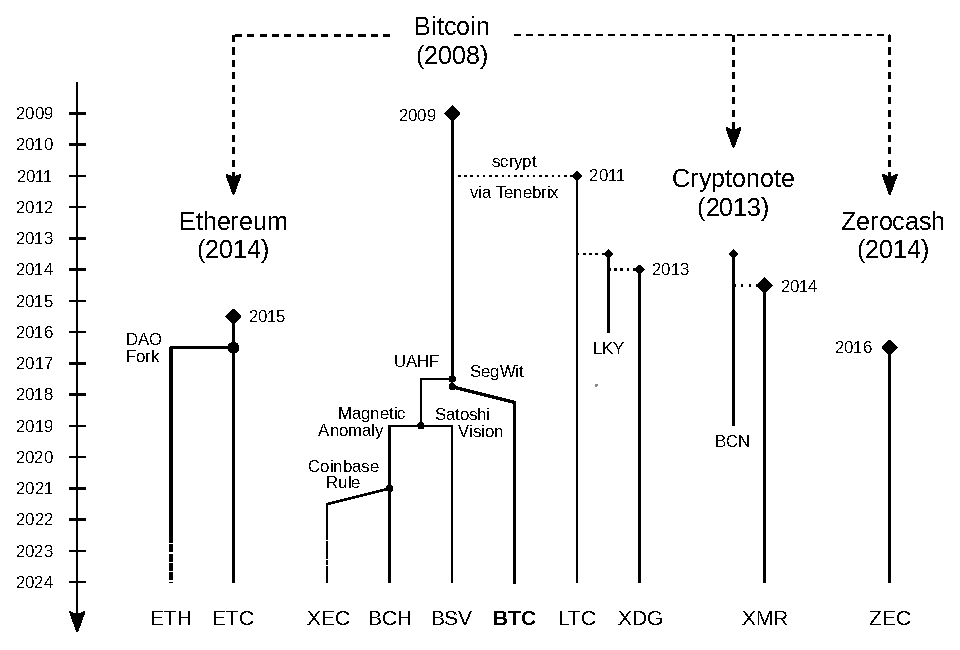
\includegraphics[scale=0.68]{img/bitcoin-forks-tree.eps}
  \caption{Variations conceptuelles, modifications logicielles et forks de consensus de Bitcoin.}
  \label{fig:bitcoin-forks-tree}
\end{figure}